\section{Анализ требований к программному средству и разработка функциональных требований}
\label{sec:domain}

\subsection{Функциональная модель программного средства}
\label{sec:domain:model}

Функциональная модель программного средства представлена в виде\linebreakсхемы алгоритма процесса обучения и диаграммы вариантов использования и информационной модели предметной области. Варианты использования отражают функциональность системы в ответ на внешние воздействия с точки зрения получения значимого результата для пользователей. Информационная модель предметной области в дальнейшем будет использоваться при проектировании базы данных для программного средства.

\subsubsection{} Анализ процесса образования
\label{sec:domain:model:deeds}

Перед началом проектирования необходимо проанализировать процесса образования. В связи с отсутствием опыта преподавания у исполнителя данного дипломного проекта выглядит целесообразным проведение данного анализа с точки зрения студента. Результат анализа представлен в виде схемы алгоритма на рисунках \ref{fig:domain:model:deeds:student_algorithm} и \ref{fig:domain:model:deeds:student_algorithm_2}. Схема ограничивается процессом обучения в семестре и не включает проверку знаний в виде зачетов и экзаменов, завершающих обучение по дисциплине.

\begin{figure}
\centering
	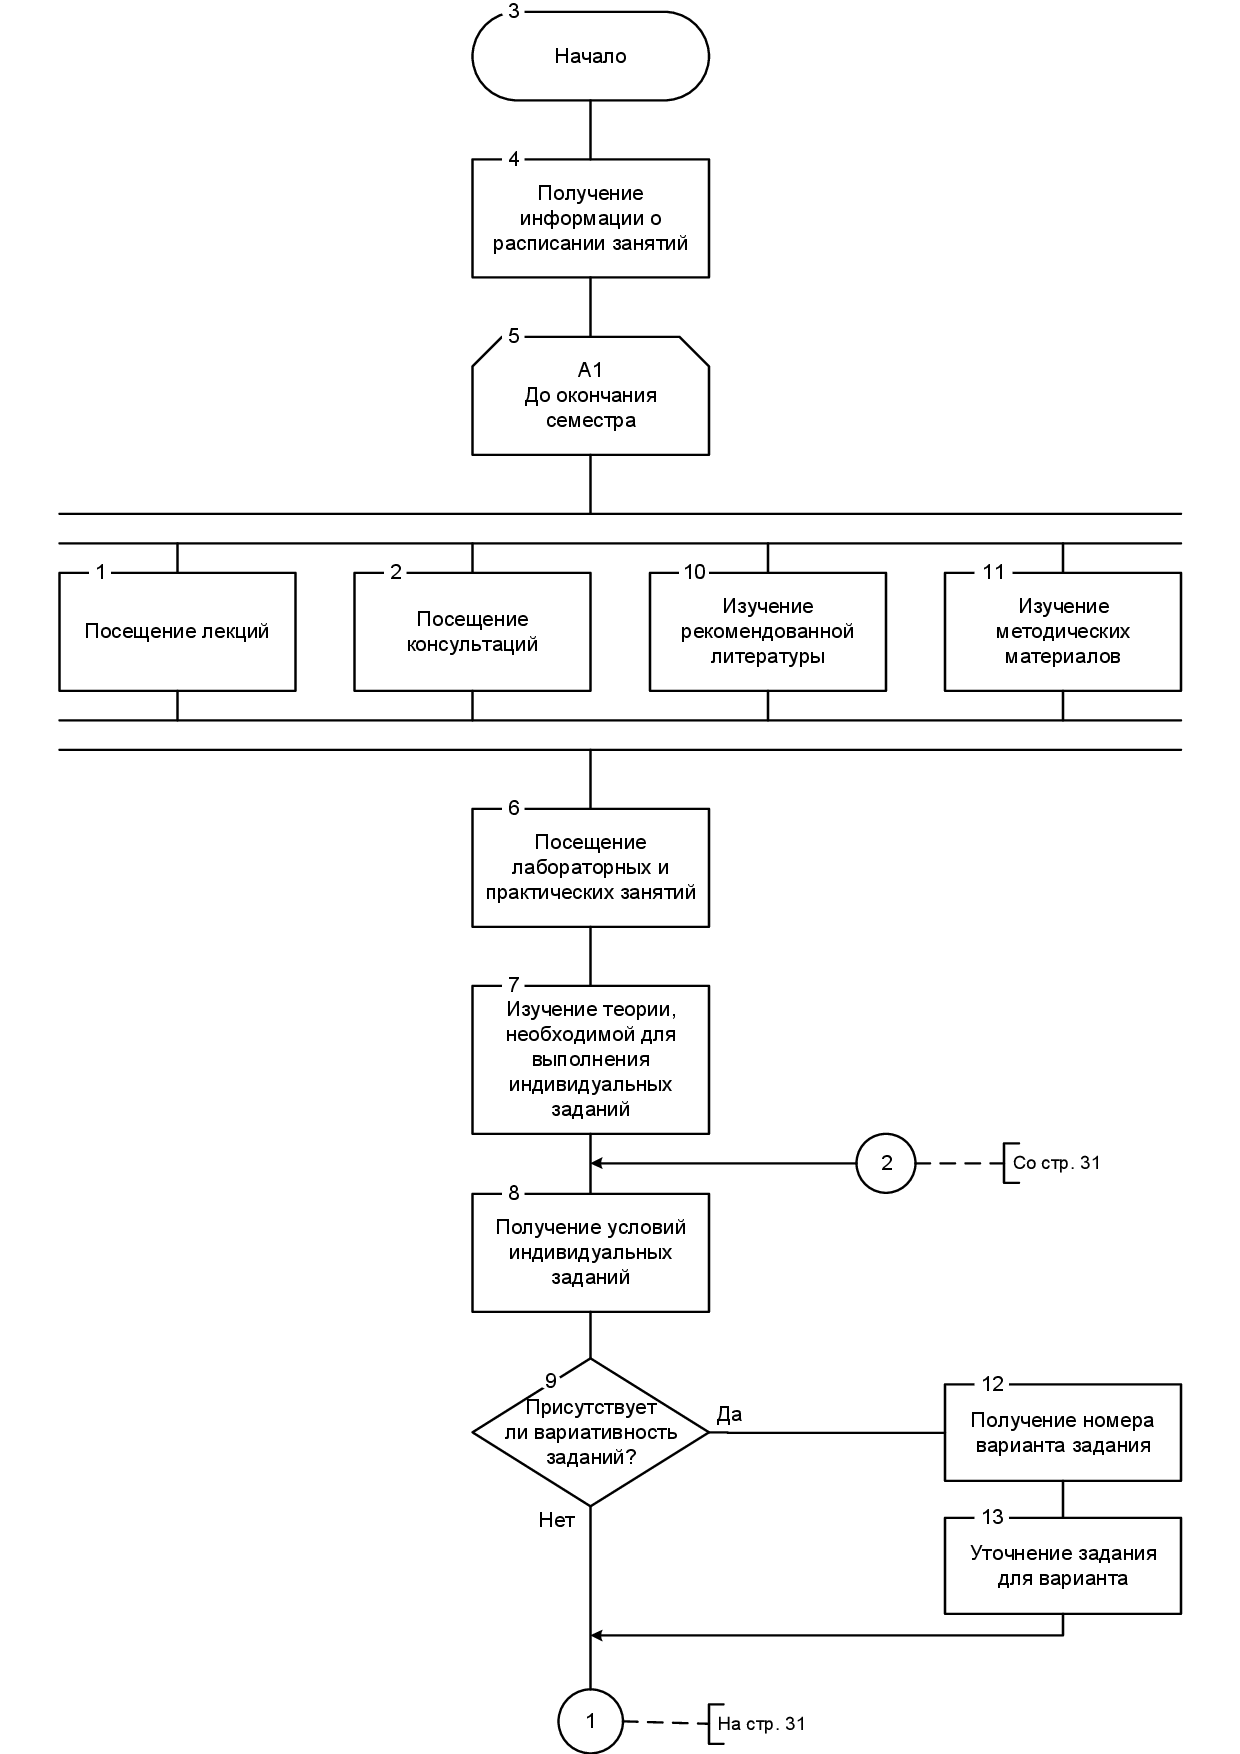
\includegraphics[scale=0.815]{student_algorithm.png}
	\caption{Схема алгоритма процесса образования с точки зрения студента}
	\label{fig:domain:model:deeds:student_algorithm}
\end{figure}

\begin{figure}
\ContinuedFloat
\centering
	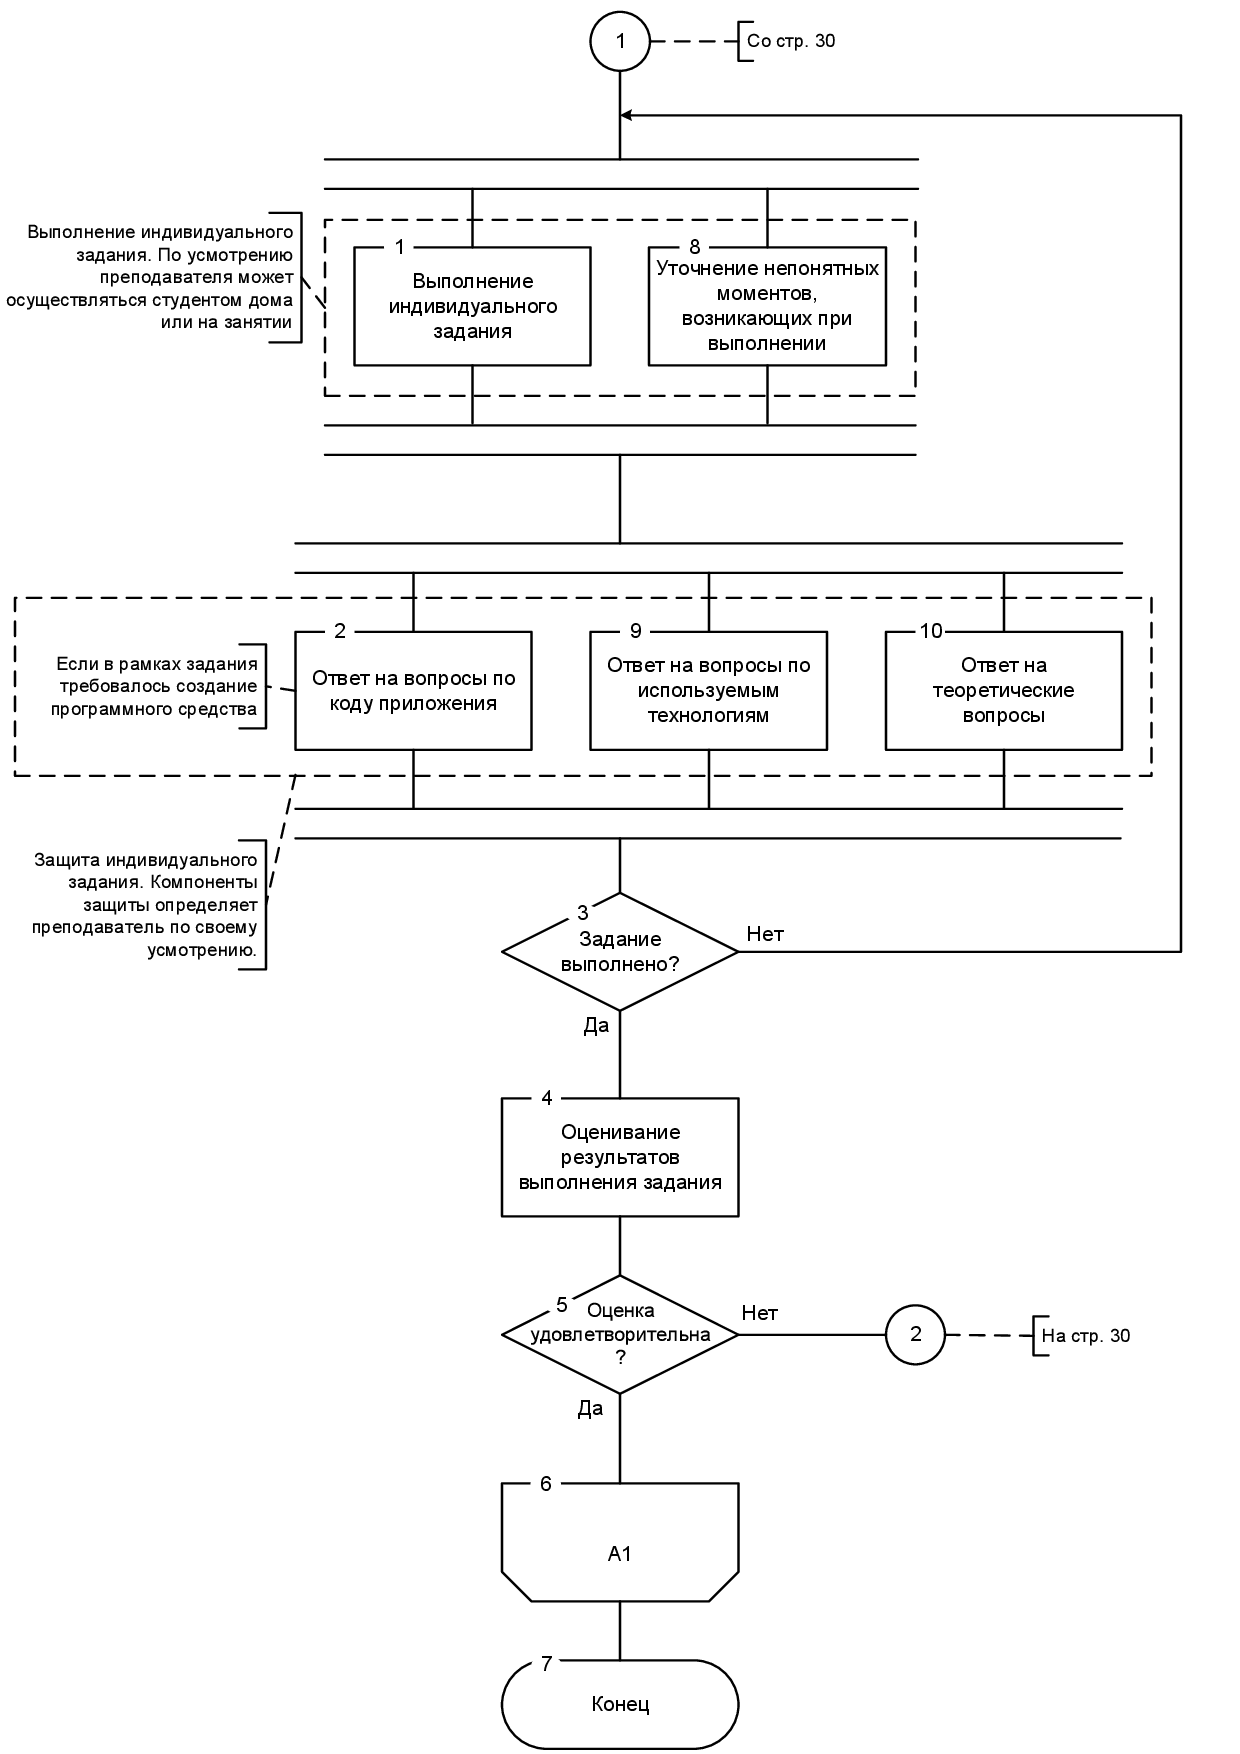
\includegraphics[scale=0.815]{student_algorithm_2.png}
	\caption{Схема алгоритма процесса образования с точки зрения студента (окончание)}
	\label{fig:domain:model:deeds:student_algorithm_2}
\end{figure}

Одной из особенностей данной схемы является цикличность, с которой выполняется процесс обучения. Цикл начинается изучением некоторой теории по дисциплине, затем на практическом или лабораторном занятии преподаватель разъясняет некоторые сложные моменты, которые могут возникнуть при выполнении индивидуальных заданий, выдаёт условие заданий, а также вариант. Студент на занятии или дома выполняет задание. После этого на одном из занятий или вне их происходит защита результатов выполнения заданий. После этого происходит оценивание результатов преподавателем. Если задание выполнено не полностью, то оно отправляется на доработку. Если же оценка не является удовлетворительной, то преподаватель вправе выдать новое задание.

Таким образом на схеме алгоритма приведен типичный вариант обучения студента, который широко практикуется в университетах и практически никак не автоматизирован. Программное средство, разработка которой ведется в данном дипломном проекте, не изменит устоявшейся системы сразу, однако значительно упростит выполнение многих ее этапов.

\subsubsection{} Варианты использования программного средства
\label{sec:domain:model:use_cases}

В результат анализа предметной области и существующих аналогов можно сделать вывод, что проектируемое программное средство должно поддерживать набор функций, который бы полностью удовлетворял потребности пользователей с точки зрения обычной социальной сети, а также специфические функции, необходимые только для мотоцикслистов. Выделим следующие:

\begin{itemize}
	\item \emph{Интеграция с существуюшими социальными сетями}, которая позволит производить авторизацию в приложении с использованием существующих учетных записей пользователей из других социальных сетей.
	\item \emph{Сообщения} позволяют обмениваться информацией, находить друзей и единомышленников.
	\item \emph{Публикации} представляют собой записи, которые могут содержать фото, видеофайлы и текст записи с хештегами.
	\item \emph{Управления мотопарком}. Возможность прикрепления информации о мотопарке пользователя: создание публикаций с указанием технических характеристик мотоциклов, а также удаление и редактирование данной информации.
	\item \emph{Гараж}. Страница отображает информацию о мотопарке пользователя: фотографии, видео, технические характеристики, комментарии других пользователей, лайки. 
	\item \emph{Профиль пользователя}. Отдельная страница, которая отображает краткую информацию о человеке, его мотопарке, а также содержит секцию с публикациями пользователя.
	\item \emph{Личный блог}. Возможность ведения личного блога предусматривает создание публикаций с пометкой <<Запись>>. Данные публикации будут отмечены специальным индефикатором в секции со всеми публикациями (профиль пользователя).
	\item \emph{Управление друзьями и подписчиками}. Возможность отправки и отмены запросов на добавления в друзья, поиск других пользователей.
	\item \emph{Отправка оповещений}. Возможность отправки оповещений о состоянии приложения, а также о действиях других пользователей (комментирование публикакации, добавление лайков на запись).
	\item \emph{Настройка учетной записи} позволит изменять информацию о пользователе, прикреплять ссылки на другие социальные сети, устанавливать настройки приватности, изменять пароль.
	\item \emph{Лента}. Отдельная страница, которая представляет собой список публикаций. Следует предусмотреть ее разграничение на публикации, размещенные только друзьями, и на популярные, которые получили больше всего лайков в приложении.
	\item \emph{Режим катания на мотоцикле}. Возможность переключения в данный режим указывет на то, что пользователь в данный момент едет на мотоцикле или изъявляет желание покататься.
	\item \emph{Карта}. Отдельный раздел приложения, который представляет собой страницу, содержащую карту с геолокацией, на которой отмечены друзья, у которых установлен режим катания на мотоцикле, а также метки. Следует предусмотреть функцию возврата фокуса к текущему местоположению, а также поиск друзей.
	\item \emph{Метки}. Специальные маркеры на карте, которые будут служить инструментом предупреждения других пользователей об опаснастях и чрезвычайных ситуациях на дороге.
	\item \emph{Маячок}. Возможность отправки специального сигнала в виде текстового сообщения другу, который в данный момент катается на мотоцикле, т.е. отмечен на карте.
	%которые отображаются на карте, бывают двух типов: <<Предупреждение>> и <<SOS>>. При установке последнего пользователем его друзьям должно приходить оповещение с оповещение должно приходить 
\end{itemize}

Диаграмма вариантов использования, разработанная с использованием нотации \uml, представлена на рисунке~\ref{fig:domain:model:use_cases:model}.

\begin{figure}[ht]
\centering
	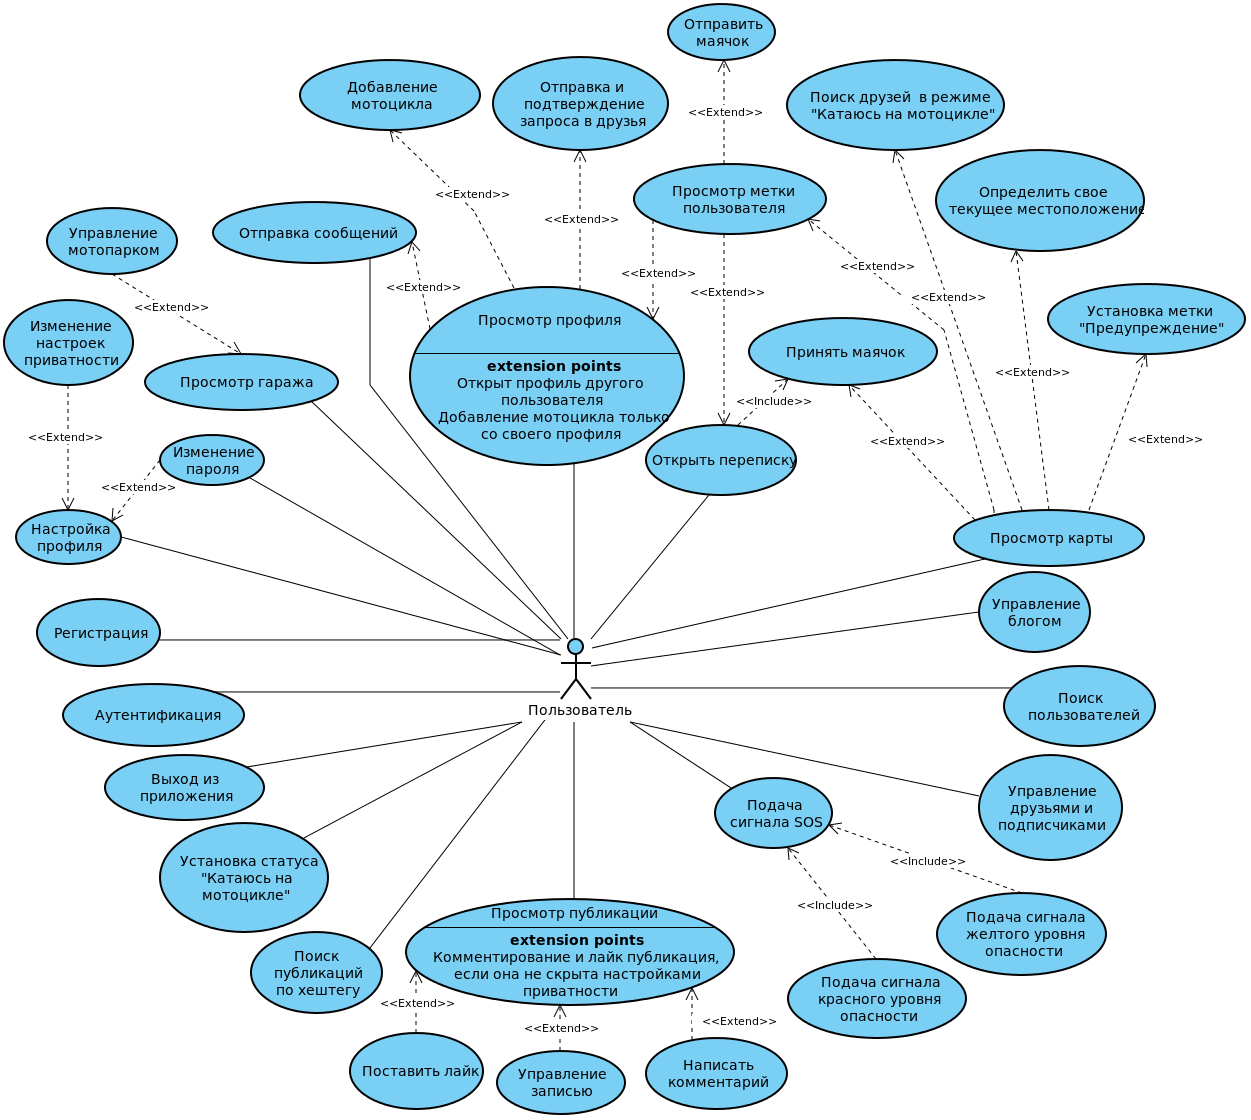
\includegraphics[scale=0.5]{use-case-diagram.png}
	\caption{Диаграмма вариантов использования ПС}
	\label{fig:domain:model:use_cases:model}
\end{figure}

Рассмотрим подробно представленные на рисунке прецеденты.

\emph{Регистрация, аутентификация и авторизация}. В приложения планируется реализация собственной системы авторизации, а также возможность регистрации с помощью учетных записей от других социальных сетей (\facebook~и \vk.).

После регистрации пользователь получает доступ к \emph{поиску пользователей}, системе \emph{сообщений}. Однако, для участия в учебном процессе необходимо \emph{подтверждение роли}. Только после подтверждения преподаватели получают доступ к предметам, которые они преподают, а студенты зачисляются в группы. 



\subsubsection{} Разработка инфологической модели базы данных
\label{sec:domain:model:db}

Исходя из необходимости использования в проектируемом приложении базы данных, разработаем ее инфологическую модель. Для ее создания будем использовать расширение диаграммы классов \uml, предназначенное для моделирования баз данных. Полученная диаграмма (рисунок~\ref{fig:domain:model:db:model}) будет являться моделью базы данных инфологического уровня~\cite{kulikov_db_workbook}.

\begin{figure}
\centering
	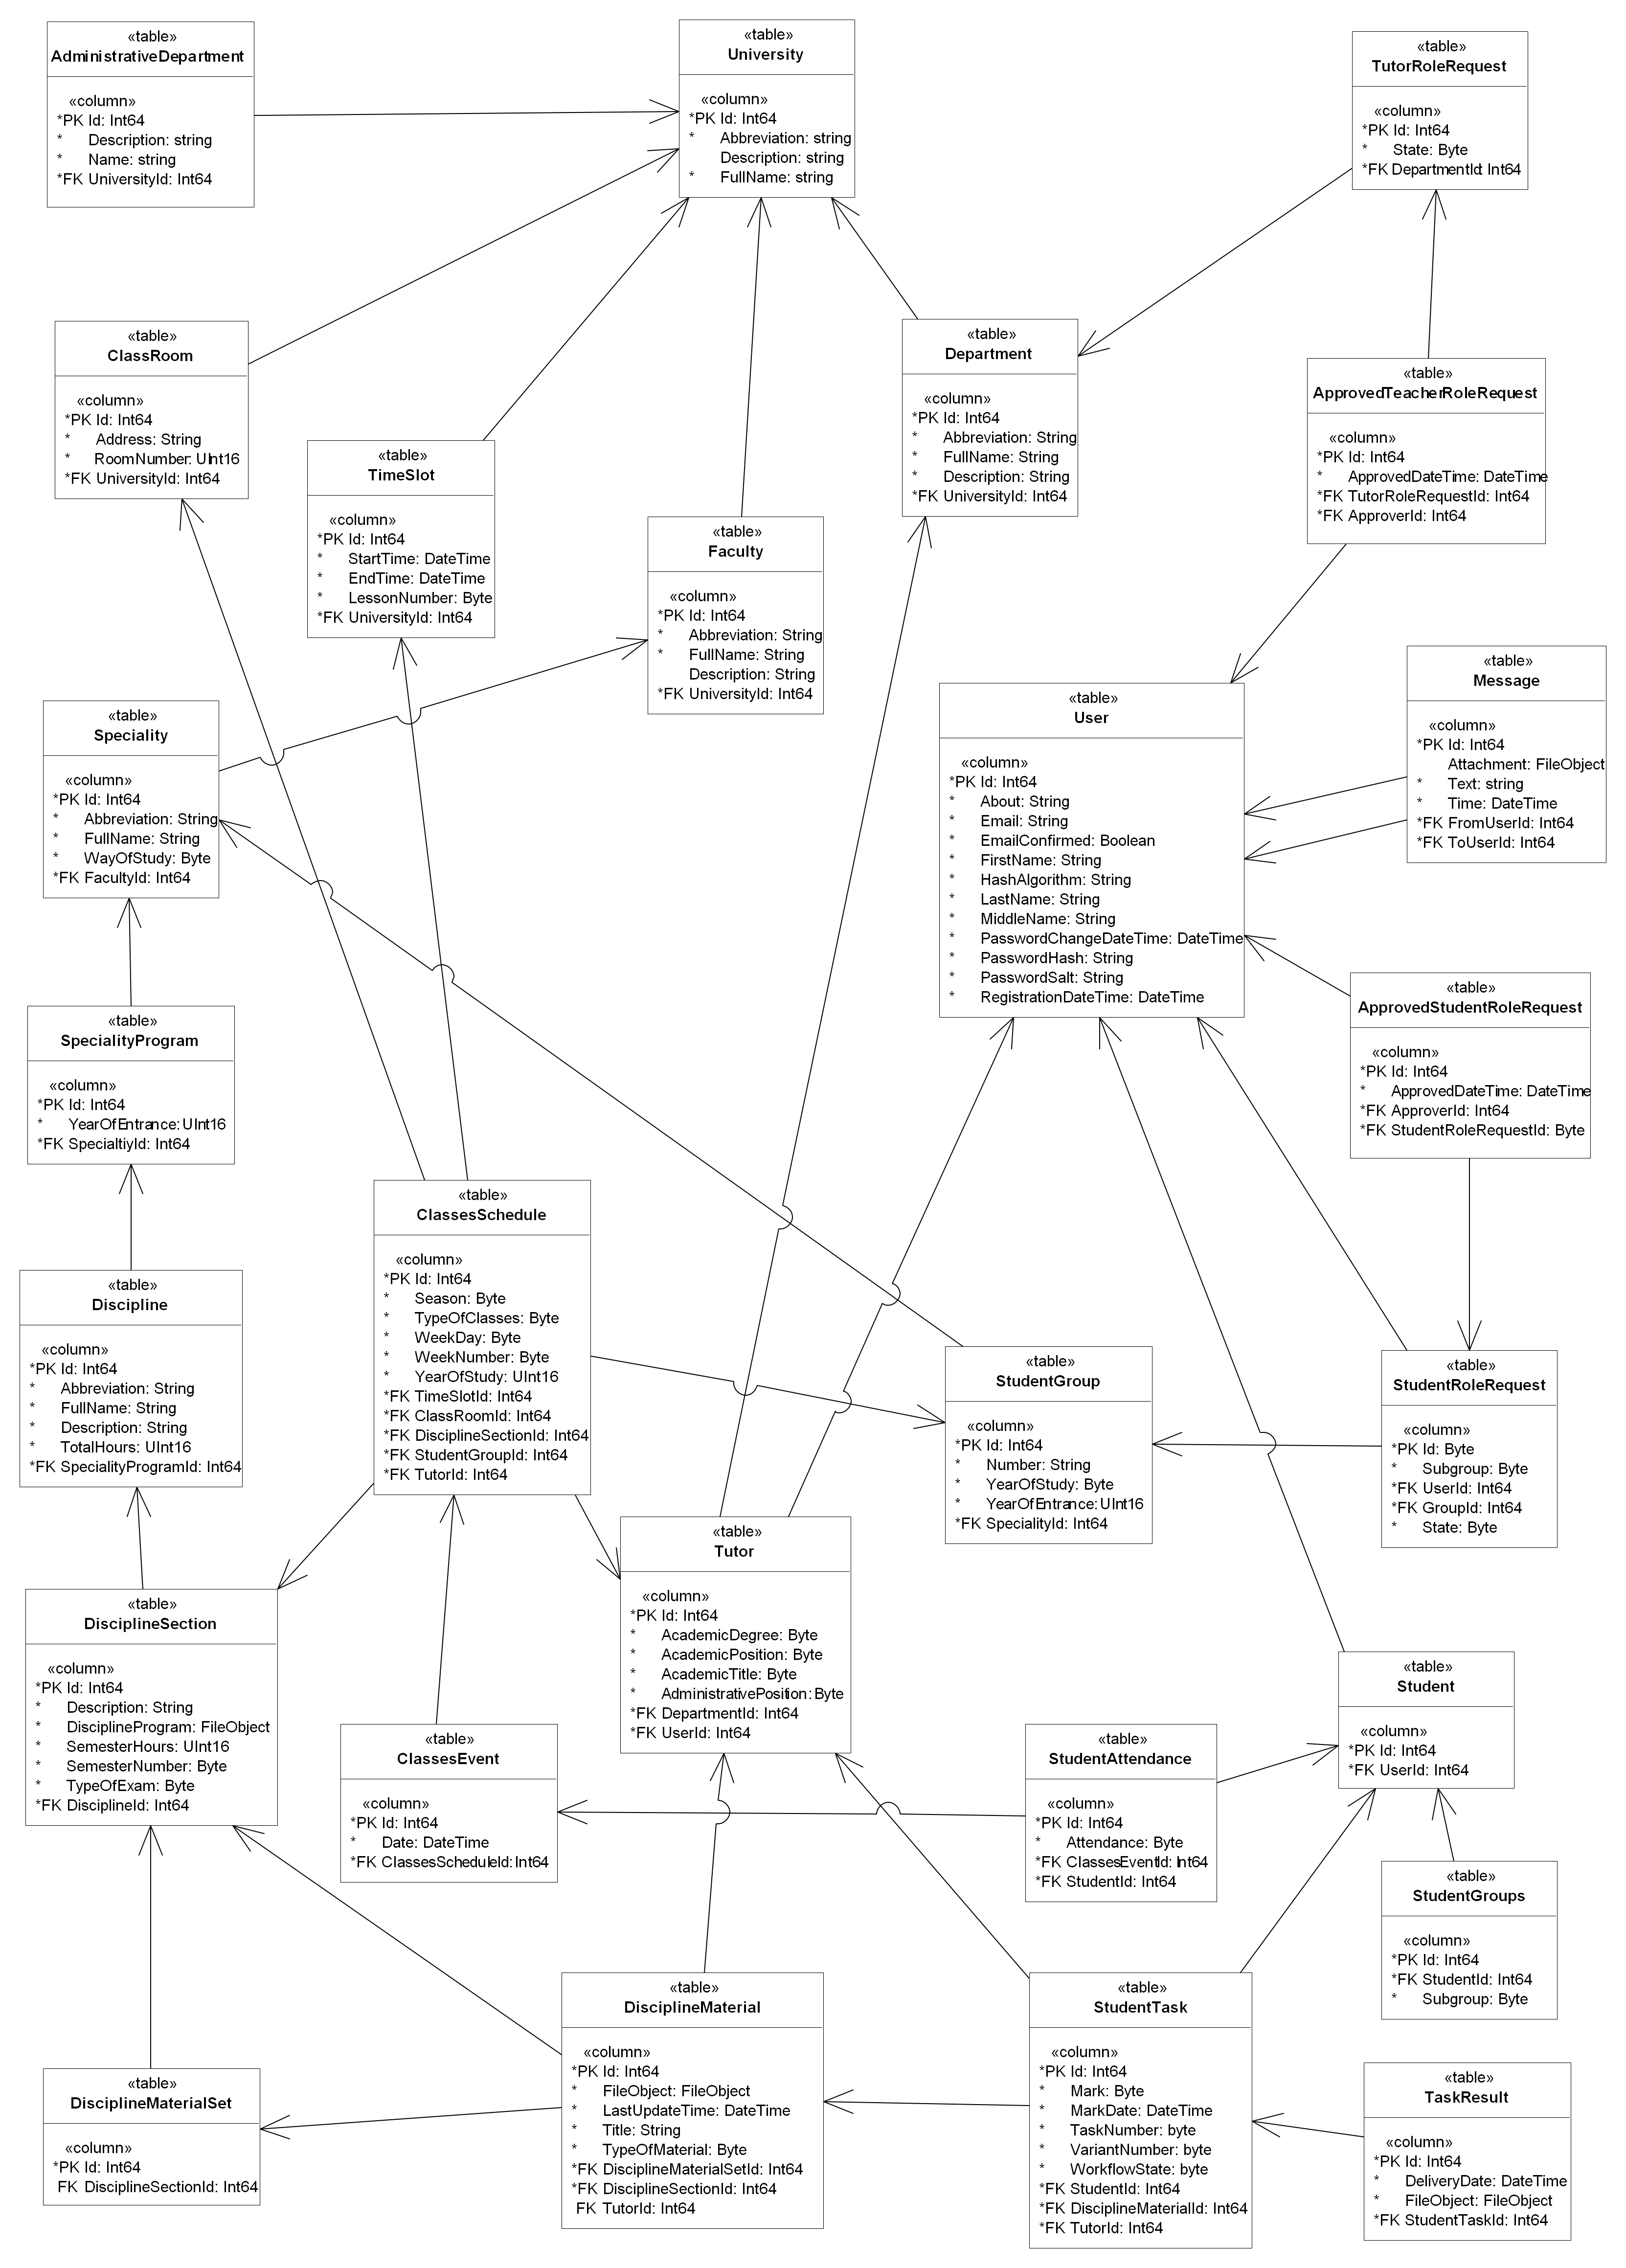
\includegraphics[scale=0.146]{domain_information_model.png}
	\caption{Инфологическая модель базы данных}
	\label{fig:domain:model:db:model}
\end{figure}

Одной из особенностей разработанной модели является отсутствие в ней типов перечисления. Вместо них повсеместно (например, в таблицах Speciality, TutorRoleRequest, StudentAttendance, DisciplineMaterial и некоторых других) используется целочисленный тип Byte. Это связано с особенностями планируемой к использованию СУБД. По сути, это заглушки, вместо которых будут использоваться соответствующие типы перечислений.

Можно заметить, что все остальные используемые типы данных соответствуют типам языка программирования \csharp. Причиной использования данной нотации в модели является то, что для доступа к базе данных будет использоваться клиентская библиотека, реализованная для платформы \dotnet. Кроме того, данная библиотека является очень важным ограничением, которое влияет на выбор архитектуры и используемые технологии.

В информационной модели предусмотрены возможности для обеспечения безопасности аутентификации и авторизации: в таблице User предусмотрены поля для хранения хешированного пароля и соли, и, вдобавок, строки с названием хеширующего алгоритма.

Предполагается, что в проектируемой системе не будет возможности изменения набора ролей -- существующие выбранные роли очень жестко привязываются к структуре БД. С другое стороны, предметная область и не предполагает выделения большого количества ролей, а практически любое действующее лицо можно свести к одной из существующих.

В проектируемой системе предполагается существование иерархии сущностей. На вершине находятся университеты; предполагается поддержка многих ВУЗов одной системой. Университеты имеют в своем составе следующие единицы: административные отделы (используются в информа\-ционно-справочных целях), факультеты, кафедры.

\subsection{Разработка спецификации функциональных требований}
\label{sec:domain:specification}

С учетом требований, определенных в подразделе \ref{sec:analysis:specification}, представим детализацию функций проектируемого ПС.

\subsubsection{} Функция регистрации
\label{sec:domain:specification:signup}

Функция регистрации должна быть реализована с учетом следующих требований:

\begin{enumerate}
	\item Процесс регистрации инициируется пользователем системы (на рисунке~\ref{fig:domain:model:use_cases:model} представлен в виде роли <<Гость>>).
	\item Функция реализуется собственными средствами без обращения к вне\-ш\-ним поставщикам.
	\item Для регистрации пользователь обязан предоставить адрес электронной почты и установить пароль.
	\item Правильность предоставленного адреса электронной почты должна проверяться путем отправки письма со ссылкой, переход по которой означает подтверждение пользователя.
	\item Хранение пароля допускается только в хешированном виде; применяющийся алгоритм должен по криптостойкости быть равным или превосходить алгоритмы семейства SHA-2. Использование соли обязательно.
	\item Должна быть предусмотрена возможность смены пароля и электронной почты после регистрации. Правильность нового адреса почты проверяется отправкой на него письма с подтверждающей ссылкой.
\end{enumerate}

\subsubsection{} Функция аутентификации
\label{sec:domain:specification:authentication}

Функция аутентификации должна быть реализована с учетом следующих требований:

\begin{enumerate}
	\item Инициатором является пользователь, при этом ему необходимо предоставить адрес электронной почты и пароль, заданные при регистрации.
	\item Должна быть реализована возможность повторной аутентификации пользователя без необходимости ввода какой-либо информации.
	\item Должна быть реализована возможность восстановления пароля:
	\begin{enumerate}
		\item Для восстановления пароля пользователь должен предоставить адрес электронной почты, зарегистрированный в системе.
		\item На предоставленный адрес высылается уникальная ссылка.
		\item После перехода пользователем по данной ссылке ему предоставляется возможность установить новый пароль.
	\end{enumerate}
\end{enumerate}

\subsubsection{} Система ролей
\label{sec:domain:specification:roles}

При реализации системы ролей следует учесть требования:

\begin{enumerate}
	\item Должны быть реализованы следующие роли:
	\begin{enumerate}
		\item студент;
		\item преподаватель;
		\item администратор факультета;
		\item администратор университета.
	\end{enumerate}
	\item Для роли администратор университета должна быть реализована возможность назначения любого пользователя администратором факультета.
	\item Для получения роли студента или преподавателя у пользователей дол\-ж\-на быть возможность создать соответствующую заявку. Подтверждение заявок возлагается на администраторов факультетов.
	\item При подаче заявки на роль студента необходимо предоставить информацию о группе, в которой состоит пользователь.
	\item При подаче заявки на роль преподавателя необходимо указать кафедру, сотрудником которой является пользователь.
	\item Должна быть реализована возможность наличия у одного пользователя нескольких необязательно разных ролей.
\end{enumerate}

\subsubsection{} Функция просмотра расписания
\label{sec:domain:specification:agenda}

Просмотр расписания входит в число основных функций разрабатываемого приложения. При реализации данной функции необходимо учесть следующие требования:

\begin{enumerate}
	\item Необходимо обеспечить отображение расписания занятий в виде последовательного списка, отсортированного в порядке возрастания даты и времени их начала.
	\item Расписание должно отображаться на основании указанной группы и подгруппы (для студентов) и указанного полного имени (для преподавателей). В случае, когда подгруппа студента не указана, то должно отображаться расписание всех подгрупп.
	\item В расписании для каждого занятия должна быть отображена следующая информация:
	\begin{enumerate}
		\item время начала занятия;
		\item время окончания занятия;
		\item название (аббревиатура) предмета;
		\item тип занятия;
		\item аудитория проведения занятия (с указанием учебного корпуса);
		\item фамилия и инициалы преподавателя (для студентов) или номера групп (для преподавателей).
	\end{enumerate}
	\item Расписание должно автоматически загружаться с использованием открытого API университетов.
\end{enumerate}

\subsubsection{} Функция просмотра предметов
\label{sec:domain:specification:subjects}

Функция просмотра предметов должна быть реализована с учетом следующих требований:

\begin{enumerate}
	\item У студентов и преподавателей должна быть возможность просмотра соответственно изучаемых и преподаваемых дисциплин.
	\item В списке дисциплин должна быть отображена следующая\linebreak информация:
	\begin{enumerate}
		\item аббревиатура дисциплины;
		\item фамилии преподавателей или номера групп;
		\item общее число часов, отводимое планом.
	\end{enumerate}
\end{enumerate}

\subsubsection{} Функция управления заданиями
\label{sec:domain:specification:tasks}

Функция управления заданиями также является ключевой. При ее реализации должны быть учтены следующие требования:

\begin{enumerate}
	\item У преподавателя должна быть возможность создания, модификации и удаления индивидуальных заданий для студентов.
	\item При создании индивидуального задания необходимо указать его тип, а также предоставить файл с условием.
	\item Студенты должны иметь возможность отправлять результаты выполнения заданий с помощью проектируемой системы.
	\item В случае отправки заданий на проверку они должны помещаться в очередь.
	\item Преподаватель должен иметь возможность просматривать полученные от студентов результаты выполнения и оценивать или отклонять их.
	\item Оценивание работ должно производиться по правилам, принятых в ВУЗах: отметки от 10 до 4, а также зачтено. Отметки ниже указанных семантически означают отклонение работы и системой реализовываться не должны.
	\item В случае отклонения результатов выполнения задания (отправки на доработку) или в других случаях студент должен иметь возможность повторно загружать результаты выполнения заданий; при этом должна формироваться их история.
	\item Преподаватели также должны иметь возможность загружать учебно-методические материалы, литературу, которая может быть полезной для студентов.
	\item Студенты должны иметь возможность просматривать прогресс по\linebreakвсем индивидуальным заданиям по всем предметам на одной странице приложения.
	\item Преподаватели должны иметь возможность просматривать количество работ в очереди на проверку на одной странице.
\end{enumerate}

\subsubsection{} Функция обмена сообщениями
\label{sec:domain:specification:messages}

Функция коммуникации должна реализовывать следующие требования:

\begin{enumerate}
	\item Должна быть возможность отправки сообщений одного пользователя другому.
	\item История сообщений должна быть представлена в виде диалогов, где отображается текст сообщения, имя пользователя и время отправки сообщения.
	\item Должна быть возможность прикрепления некоторого файла к сообщению.
	\item У пользователей должна быть возможность создания объявлений, которые были бы видны всем другим пользователям. Их история должна отображаться в виде доски объявлений.
\end{enumerate}

\subsubsection{} Функция просмотра истории студента
\label{sec:domain:specification:student_history}

Следующая группа требований относится к деятельности преподавателя:

\begin{enumerate}
	\item У преподавателя должна быть возможность проверки посещаемости студентами занятий. Проверка должна быть реализована в виде ручного выставления преподавателем отметок о присутствии.
	\item Отметки о посещаемости, а также о выполнении индивидуальных заданий должны отображаться в виде таблиц по каждой группе. 
	\item Должна быть возможность просмотра данных таблиц другими преподавателями, если они преподают один и тот же предмет (но, возможно, разные типы занятий).
\end{enumerate}
